\documentclass[journal]{vgtc}                % final (journal style)
%\documentclass[review,journal]{vgtc}         % review (journal style)
%\documentclass[widereview]{vgtc}             % wide-spaced review
%\documentclass[preprint,journal]{vgtc}       % preprint (journal style)

%% Uncomment one of the lines above depending on where your paper is
%% in the conference process. ``review'' and ``widereview'' are for review
%% submission, ``preprint'' is for pre-publication, and the final version
%% doesn't use a specific qualifier.

%% Please use one of the ``review'' options in combination with the
%% assigned online id (see below) ONLY if your paper uses a double blind
%% review process. Some conferences, like IEEE Vis and InfoVis, have NOT
%% in the past.

%% Please note that the use of figures other than the optional teaser is not permitted on the first page
%% of the journal version.  Figures should begin on the second page and be
%% in CMYK or Grey scale format, otherwise, colour shifting may occur
%% during the printing process.  Papers submitted with figures other than the optional teaser on the
%% first page will be refused. Also, the teaser figure should only have the
%% width of the abstract as the template enforces it.

%% These few lines make a distinction between latex and pdflatex calls and they
%% bring in essential packages for graphics and font handling.
%% Note that due to the \DeclareGraphicsExtensions{} call it is no longer necessary
%% to provide the the path and extension of a graphics file:
%% \includegraphics{diamondrule} is completely sufficient.
%%
\ifpdf%                                % if we use pdflatex
  \pdfoutput=1\relax                   % create PDFs from pdfLaTeX
  \pdfcompresslevel=9                  % PDF Compression
  \pdfoptionpdfminorversion=7          % create PDF 1.7
  \ExecuteOptions{pdftex}
  \usepackage{graphicx}                % allow us to embed graphics files
  \DeclareGraphicsExtensions{.pdf,.png,.jpg,.jpeg} % for pdflatex we expect .pdf, .png, or .jpg files
\else%                                 % else we use pure latex
  \ExecuteOptions{dvips}
  \usepackage{graphicx}                % allow us to embed graphics files
  \DeclareGraphicsExtensions{.eps}     % for pure latex we expect eps files
\fi%

%% it is recomended to use ``\autoref{sec:bla}'' instead of ``Fig.~\ref{sec:bla}''
\graphicspath{{figures/}{pictures/}{images/}{./}} % where to search for the images

\usepackage{microtype}                 % use micro-typography (slightly more compact, better to read)
\PassOptionsToPackage{warn}{textcomp}  % to address font issues with \textrightarrow
\usepackage{textcomp}                  % use better special symbols
\usepackage{amsmath}
%\usepackage{amsbsy}
%\usepackage{amsfonts}
% or
\usepackage{amssymb}
\usepackage{hyperref}
\usepackage{mathptmx}                  % use matching math font
\usepackage{times}                     % we use Times as the main font
\renewcommand*\ttdefault{txtt}         % a nicer typewriter font
\usepackage{cite}                      % needed to automatically sort the references
\usepackage{tabu}                      % only used for the table example
\usepackage{booktabs}                  % only used for the table example
%% We encourage the use of mathptmx for consistent usage of times font
%% throughout the proceedings. However, if you encounter conflicts
%% with other math-related packages, you may want to disable it.

%% In preprint mode you may define your own headline.
%\preprinttext{To appear in IEEE Transactions on Visualization and Computer Graphics.}

%% If you are submitting a paper to a conference for review with a double
%% blind reviewing process, please replace the value ``0'' below with your
%% OnlineID. Otherwise, you may safely leave it at ``0''.
\onlineid{0}

%% declare the category of your paper, only shown in review mode
\vgtccategory{Research}
%% please declare the paper type of your paper to help reviewers, only shown in review mode
%% choices:
%% * algorithm/technique
%% * application/design study
%% * evaluation
%% * system
%% * theory/model
\vgtcpapertype{algorithm/technique}

%% Paper title.
\title{Neural Network Weight Flow Visualization}

%% This is how authors are specified in the journal style

%% indicate IEEE Member or Student Member in form indicated below
\author{Lindsey Sawatzky and Volodymyr Kozyr}

%other entries to be set up for journal
%\shortauthortitle{Biv \MakeLowercase{\textit{et al.}}: Global Illumination for Fun and Profit}
%\shortauthortitle{Firstauthor \MakeLowercase{\textit{et al.}}: Paper Title}

%% Abstract section.
\abstract{The prevalence of neural networks in a broad range of applications has opened up an important field in visualization, where we seek to explain and diagram the complexities of these neural network systems.
Many different approaches to this have been undertaken, but as far as these authors are aware non attempt to visualize the flow of weights through these networks in a elucidating way.
We make such an attempt by diagramming not matrices or activations, but rather weights and their changes through the computational graph.
Although the relatively high dimensionality and mass of this data can be quite daunting, we use several novel techniques to that help the user to focus into the interesting aspects of the neural network and visualize the weights in a meaningful and informative manner.
} % end of abstract

%% Keywords that describe your work. Will show as 'Index Terms' in journal
%% please capitalize first letter and insert punctuation after last keyword
\keywords{Neural Network Visualization, LSTM, Weight Vector, Word Embedding, t-SNE.}

%% ACM Computing Classification System (CCS).
%% See <http://www.acm.org/class/1998/> for details.
%% The ``\CCScat'' command takes four arguments.

%\CCScatlist{ % not used in journal version
% \CCScat{K.6.1}{Management of Computing and Information Systems}%
%{Project and People Management}{Life Cycle};
% \CCScat{K.7.m}{The Computing Profession}{Miscellaneous}{Ethics}
%}

%% Uncomment below to include a teaser figure.
\teaser{
  \centering
  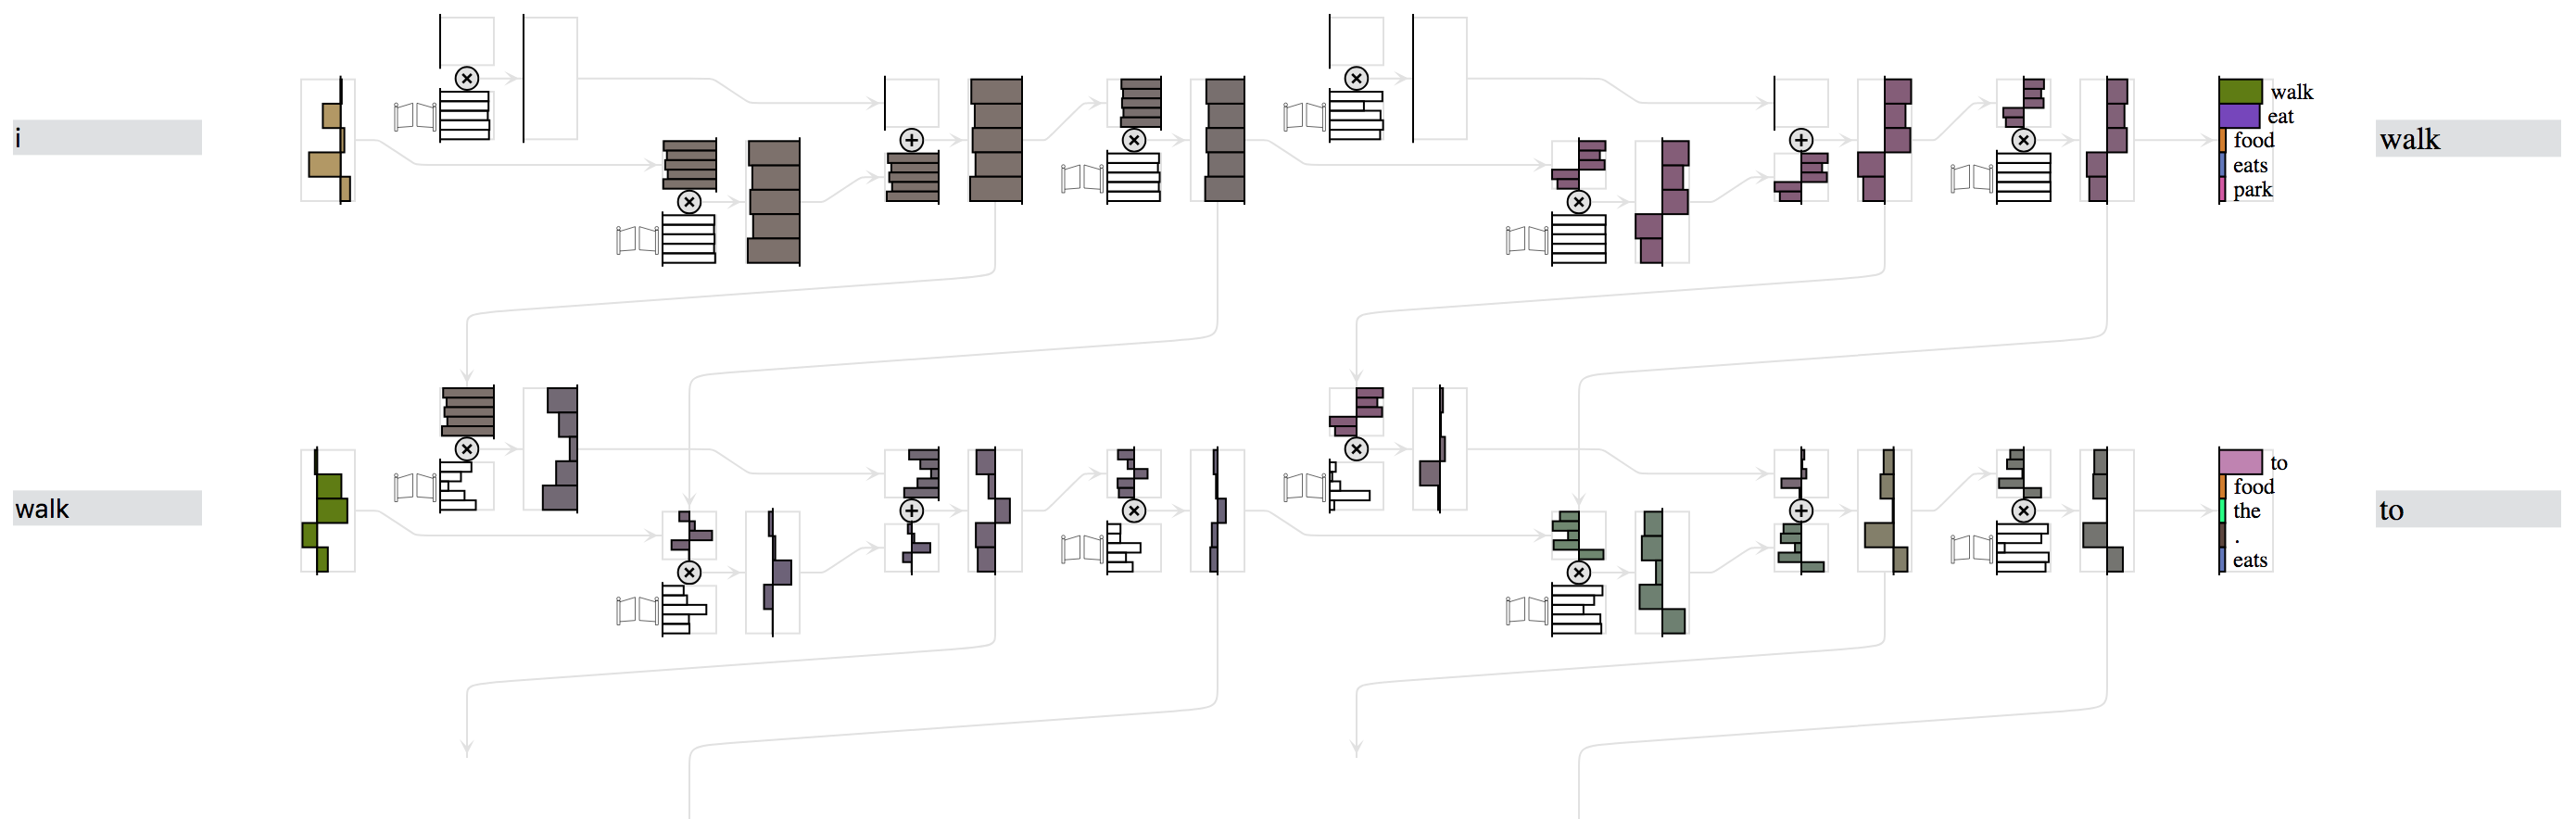
\includegraphics[width=\linewidth]{2layers.png}
  \caption{Two timesteps of the Neural Network Weight Flow Visualization}
    \label{fig:teaser}
}

%% Uncomment below to disable the manuscript note
\renewcommand{\manuscriptnotetxt}{}

%% Copyright space is enabled by default as required by guidelines.
%% It is disabled by the 'review' option or via the following command:
% \nocopyrightspace

\vgtcinsertpkg

%%%%%%%%%%%%%%%%%%%%%%%%%%%%%%%%%%%%%%%%%%%%%%%%%%%%%%%%%%%%%%%%
%%%%%%%%%%%%%%%%%%%%%% START OF THE PAPER %%%%%%%%%%%%%%%%%%%%%%
%%%%%%%%%%%%%%%%%%%%%%%%%%%%%%%%%%%%%%%%%%%%%%%%%%%%%%%%%%%%%%%%%

\begin{document}

%% The ``\maketitle'' command must be the first command after the
%% ``\begin{document}'' command. It prepares and prints the title block.
\maketitle
%% the only exception to this rule is the \firstsection command
\section{Introduction}
Neural networks have taken one of the leading places in computing science research and the AI industry.
However, despite their proved efficacy, they are notoriously difficult to understand and debug as a result of their deep complexity, highly specialized nature, and sheer volume of data.
This has opened up a whole new area of visualization aimed at addressing the challenges.
\\
\\
Two such examples are Tensorboard ~\cite{tensorboard} and LSTMViz ~\cite{lstmviz}.
Both these tools take a aim to visualize very different aspects of neural networks, but have certainly proven useful in their own right.
\\
\\
Although these and others have enjoyed success in the area of neural network visualization, many aspects remain unexplored.
We set out to investigate one relatively unexplored area in this space, that of visualizing the weight flow of a neural network and the potential underlying semantics of those weights.




%% \section{Introduction} %for journal use above \firstsection{..} instead


\section{Domain / Users / Data / Tasks}
We narrow down the visualization task by exploring the common yet intriguing Long Short-Term Memory (LSTM) architecture~\cite{lstm}.
Although the LSTM architecture is beginning to fall out of fashion, we still feel they will be an interesting subject for the purposes of this project.
One reason for this in particular is that they have what can be roughly loosely compared to `memory', and so one of the objectives of this visualization is to help users understand what exactly this means (what exactly is being `remembered').
\\
\\
The task we set out to visualize is that of understanding, both for the purposes of learning and debugging, an LSTM neural network trained as a language model.
We explore techniques to show details around what is happening in this neural network, with the hope to uncover deeper patterns within aspects of the model and architecture itself.
\\
\\
A neural network language model is defined as a classifier trained to learn the probability distribution:

\begin{equation}
    P(w_t|context)
\end{equation}

where $w_t$ is the word to predict at timestep $t$, and the context is some representation of the current linguistic context.
The context can typically be represented as a window of previous words $w_{t-w},..,w_{t-1}$.
With a recurrent neural network, the context spans back to the beginning of the sentence $w_1,..,w_{t-1}$ through the recurrence of the network itself, and additionally includes an input word $w_{in}$ which may differ from $w_{t-1}$.

\begin{equation}
    P(w_t|w_{in},w_1,..,w_{t-1})
\end{equation}

In this model, the words of the vocabulary $V$ are encoded by a one-of-K coding.
A high dimensional embedding is trained to map words that occur in similar contexts closer in an $N << |V|$ dimensional space, while words that don't occur in similar context are trained to map farther apart in this space.
This is referred to as a word embedding, and will factor into the visual idiom design later in this work.

The recurrent units of the architecture are trained against an input corpus to minimize the error, or rather to maximize the probability (1).
Without going into too many details, the LSTM has a few key characteristics, namely that it represents and learns information that it needs to remember as weight vectors, and this information is allowed to flow or not via other weight vectors typically referred to as `gates'.
These gates sound complex, but in reality they are merely element wise multiplications, so when the gate has a value of 1 all the information is allowed through, and conversely when the gate has a value of 0 none is allowed through.
\\
\\
Finally, the end of the neural network model projects the last recurrent layer's output back into the one-of-K vocabulary space, using a softmax to create the probability distribution (1).
For more details, we refer readers to the previous works describing the neural network task and architecture itself ~\cite{lstm}~\cite{lstmlm}.
\\
\\
As this task is highly domain specific, we expect the target user group for this visualization to be researchers in the field, familiar with the fundamental concepts behind neural networks.

\section{Design of Visual Idioms and Interaction}
We incorporate a few key ideas to visualize the neural network weights and how they change and flow through the computational graph.
\begin{enumerate}
    \item Relative Magnitude Weight Widgets
    \item Colourized Weight Encoding
    \item Softmax Top-K Widget
    \item Weight Contribution Explanations
    \item Operation Zoom
\end{enumerate}
These ideas are then brought together by drawing everything together within the computational graph of the LSTM neural network.
Although the entire flow of the network is visualized, some details such as matrix multiplications and non-linearity functions aren't displayed.
The decision to focus instead on the LSTM operations and changes of the weight vectors comes out directly from the objective of the visualization task.

\subsection{Relative Magnitude Weight Widgets}
The basic idea behind this visual idiom is to show the detailed weights and how they change as a result of the various neural network computations.
Generally speaking, humans can easily follow mathematical steps when they are presented one by one with the appropriate level of detail.
Moreover, humans can also easily see the differences between 2-3 plain images, so the idea behind this visualization concept is to present small changes in logical and clear steps that aren't overwhelming.
We do so despite the underlying overwhelming nature of neural networks and the data (numeric values) they fundamentally operate on.
\\
\\
Specifically, we present the relative magnitude of the values in the $N$ dimensions of a weight vector as a horizontal bar chart, where each bar represents a single dimension of the $\mathbb{R}^N$ vector space.
These values are normalized to fit within a fixed sized box, and drawn with a 0-line for reference.
Negative weights are drawn towards the left while positives are drawn towards the right.
If the weights are all positive, then the 0-line is placed on the containing box itself, but otherwise it is placed as appropriate within the box.
The 0-line is intentionally extended a few pixels vertically beyond the containing box to visually highlight its significance.
Figure 2 shows an example of this visual idiom.

\begin{figure}[tb]
 \centering % avoid the use of \begin{center}...\end{center} and use \centering instead (more compact)
 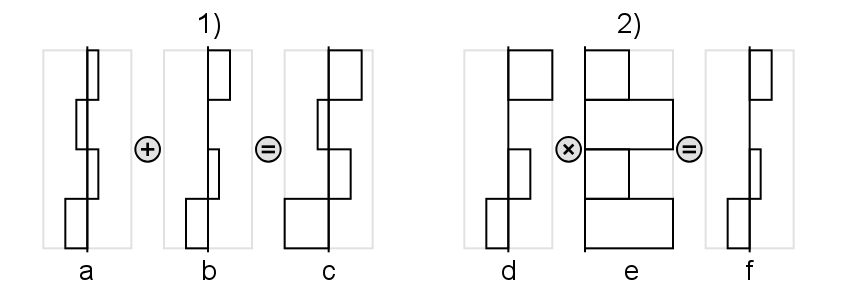
\includegraphics[width=\linewidth]{weight_diagram.png}
 \caption{Relative Magnitude Weight Widgets representing a $\mathbb{R}^4$ vector space.  1) Shows the addition of vectors \textbf{a} and \textbf{b} producing \textbf{c}.  2) Shows the multiplication of the vector \textbf{d} against the so called gate vector \textbf{e} producing \textbf{f}.}
 %\autoref{tab:vis_papers}. The image is from \cite{Isenberg:2017:VMC} and is in the public domain.}
 \label{fig:weight_add}
\end{figure}

\subsection{Colourized Weight Encoding}
Although the idea in section 3.1 produces an intuitive way to follow the changes of weights through the neural network, it still suffers from the problem of overloading the user with too much information.
Even relatively low dimensional weight vectors can become easily overwhelming.
Here we try to address this problem by thinking of the weight vector as a whole rather than a collection of values across $N$ dimensions.
\\
\\
To do so, we first leverage a technique commonly used to visualize the word embeddings of the language model neural network.
That is, a dimensionality reduction of the word embeddings into into a lower dimensional space that preserves the relative topology in the high dimensional space.
T-distributed Stochastic Neighbor Embedding (t-SNE)~\cite{tsne} has become the defacto technique for this, and so we use it to lower the dimensionality of the word embeddings.
\\
\\
Specifically, we use t-SNE to map the word embeddings into a 3-dimensional space, referred to as $C^3$ for the fact that it represents a colour cube.
The axis of this cube represent one of the three primary colours in the additive colour space: Red, Green, and Blue.
This gives a colouring to every word in the vocabulary such that words appearing together in similar contexts also have similar colours.
This colour encoding is fixed in place so that each word will consistently map to the same colour.
\\
\\
Then, we map the other weight vectors from the neural network into this colour space so that those which are most similar to the word embeddings also appear with a similar colour encoding.
This is done using a form of a force directed layout where the reference word-colour encodings are fixed in place, and the other weight vectors are fit into $C^3$ by preserving the relative distances in the high dimensional space $\mathbb{R}^N$.
\\
\\
So the operation becomes that of mapping a weight vector $\mathbf{w} \in \mathbb{R}^N$ into the colour space $C^3$.
To do so, the word embeddings $\mathbf{v} \in \R^N$ which are already mapped into colour points $\mathbf{o} \in C^3$ are used as references.
The distance $d_{v_i}$ from the weight vector $\mathbf{w}$ to each word embedding $\mathbf{v_i}$ are calculated using euclidean distance (euclidean distance is used as the basis for t-SNE, so it follows to use the same distance metric for this operation).
Then, the point $\mathbf{p}$ is fit with the following iterative equation over $t$:

\begin{equation}
\mathbf{p_t} &= \mathbf{p_{t-1}} + b_f\Delta_t    
\end{equation}
\begin{align*}
\Delta_t &= \forall_i \phi_i (d_{v_i} - d_{o_i}) \\
\phi_i &= 1 / r^{d_{v_i}} \\
d_{v_i} &= distance(\mathbf{w}, \mathbf{v_i}) \\
d_{o_i} &= distance(\mathbf{p}, \mathbf{o_i}) \\
b_f &= 1 / 1.3^f
\end{align*}
\\
where $r$ is set so the farthest target distance $d_{v_i}$ results in $\phi_i \approx .25$.
This lets $\phi_t$ represent the importance that the placement of $\mathbf{p}$ should pay respect to each target distance $d_{v_i}$, where the farthest distance is only roughly 25\% respected, and distances close to 0 are almost 100\% respected.
\\
\\
The astute reader will notice the computation of $\Delta$ is done by calculating the difference of two distances, one in $\mathbb{R}^N$ and the other in $C^3$.
Naturally, these will have very different scales, not only because of the differences in their dimensions but also simply because of the potential different in scales of values (for example, the weight vectors in $\mathbb{R}^N$ may all be values $\in [0, 1]$).
For simplicity, the equations omit a linear scaling that is performed so that comparisons between these two scales can make reasonable sense.
Specifically, the maximum target distance $d_{v_i}$ is projected to $C / 2$ while a target distance of 0 maps also to 0, and everything in between is scaled linearly between those two points.
\\
\\
$\mathbf{p}$ is set incrementally until it converges, defined as $|\Delta| < \epsilon$ for some fixed $\epsilon$.
If ever $|\Delta_t| > |\Delta_{t-1}|$, then $\Delta_t$ isn't applied and instead a back-off is introduced by incrementing $f$ and restarting the iteration at time $t$ from scratch.
\\
\\
In order to make this operation fast, we only select a random sampling of $S \leq 16$ word embeddings $\{v_1,..,v_s\}$ to use as references, which do not change after being initially sampled.
An example instance of this iterative process is shown in figure 5.

\subsection{Weight Contribution Explanations}
Since this visualization hides some of the computations that occur within the neural network, we find that sometimes it is hard to understand the transition from one dimensional value to another.
To fill this gap, we introduce an interaction that allows for the user to select a weight and visualize the contribution that all the upstream weight(s) had towards it.
In the case of looking at an element wise operation, such as the gating of the LSTM, this becomes a very trivial visualization but still helpful for consistency.
More importantly, for the un-visualized matrix multiplications this becomes an invaluable interaction that helps to describe an otherwise mathematically complex and numerous operation.
\\
\\
This interaction is enabled by by hovering over the dimensional bar of a weight vector and single clicking.
A highlight will be set on the selected value and its upstream contributor(s) will become encircled in a darker box.
Inside these, the complex mathematical operation is broken down into its constituent parts and dark highlights are superimposed on top of the values, with a directional axis the same as that of the weight vector widget itself (left encodes negative contributions, right encodes positive contributions).
\\
\\
Figure 3 part 1) demonstrates the result of this interaction.

\begin{figure}[tb]
 \centering % avoid the use of \begin{center}...\end{center} and use \centering instead (more compact)
 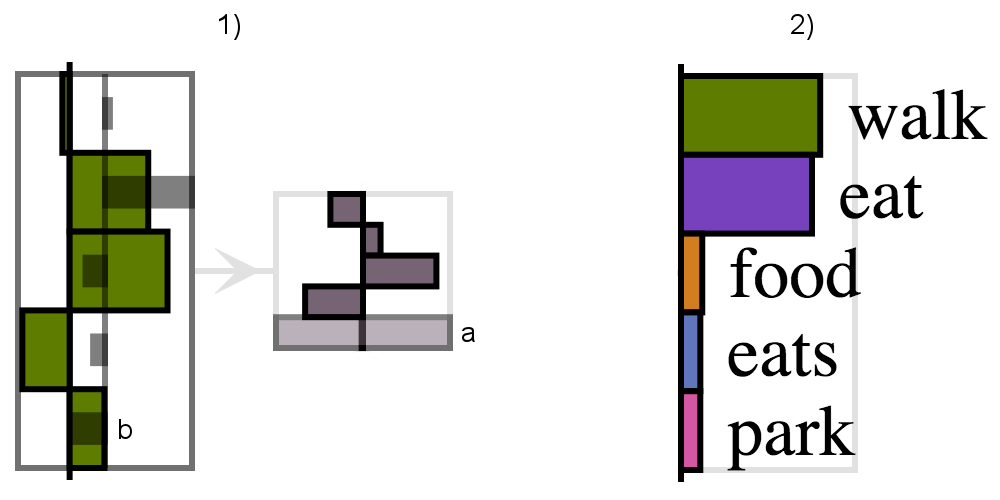
\includegraphics[width=\linewidth]{weight_explain_and_softmax.png}
 \caption{1) Explaining the final dimension (a) of the right-purple weight vector as a result of the left-green weight vector.  Despite having a value of 0, we see that in fact several positive and negative factors have contributed to the final effect.  We also see how the contribution of a value can switch, as in the example where (b) is positive but its contribution is actually negative.  2) Showing the output softmax.  The relative probabilities stand out and highlight the most likely vs. least likely words.}
 %\autoref{tab:vis_papers}. The image is from \cite{Isenberg:2017:VMC} and is in the public domain.}
 \label{fig:weight_explain}
\end{figure}

\subsection{Softmax Top-N Widget}
A simple yet effective visual element that has been incorporated is to display the final output softmax operation in the same relative magnitude weight widget style as as the rest of the visualization.
The difference however is that only the top $N$ probabilities of the softmax are displayed, and they are annotated with the corresponding encoded word (recall $N << |V|$).
Rather than drawing the entire widget in a single colour, each word is coloured separately by the same word encoding scheme as outlined in section 3.2.
This widget can be seen in Figure 3 part 2).

\subsection{Operation Zoom}
Section 3.1 outlines how we intuitively describe the changes between weights as the flow through the neural network.
Section 3.2 describes a technique that can very effectively draw a users attention to important aspects and transitions within the neural network at a macroscopic level.
However, the visualization still suffers from fundamentally cramming a lot of information into a relatively small visual space.
The final interaction we introduce to combat this tension is the ability to zoom into an operation, increasing the size of the visual elements that the user selects as interesting.
The zoom interaction nicely completes the visualization, providing an overview first and details on demand.

\section{Implementation}
Since the nature of this project was highly specialized, no existing visualization technology would have been suitable for the idioms and interactions we designed.
Thus, we built the frontend of the visualization from scratch using plain \textbf{HTML}, \textbf{Javascript}, and \textbf{D3}.
The backend server was built using python and several common libraries such as \textbf{Numpy}, \textbf{requests}, and \textbf{Sklearn}.
We used \textbf{Matplotlib} to visualize the data for diagrams and to debug the visualization implementation itself.
\\
\\
Although we had discussed the advantages to using a portable data model format such as \textbf{ONNYX}, this was ultimately not suitable for our project for two reasons.
Firstly, since we had already taken on what is certainly a large scale project, there simply was not enough time to make the implementation vendor agnostic in this way.
Secondly, since the project focuses on visualizing the actual instances of weight representations, and not the learned-but-fixed matrices of the computational graph, then ultimately the project needed to hook into a running dataflow programming library.
This certainly could be done in a vendor agnostic way via some kind of abstraction layer, but again time played an important constraint in prohibiting this option.
Therefore, we decided to use the library we were most familiar with, \textbf{Tensorflow}.
\\
\\
The neural network was trained on a sample corpus with $|V| = 20$.
As we mention in the next section, using a larger, more realistic corpus is something that must be investigated in future work on this project.
\\
\\
The entire process of designing and implementing this visualization is captured on our public \textbf{Github} project page \url{https://github.com/767-lvl/nn-wd}.
The final running visualization can be viewed on the SFU network at \url{http://eccc-nll.bigdata.sfu.ca:8889/index.html}.
Notice, at the time of writing, SFU IT services still hadn't opened up that port.

\section{Evaluation and Discussion}
To evaluate the visualization, we would like to measure its effectiveness at investigating a few aspects of the neural network language model.
In no particular order, these are:
\begin{enumerate}
    \item What portions of the neural network do the weights change most drastically?
    \item What semantic representation do the weights hold, especially the various 'memory' cells of the LSTM?
    \item If the neural network isn't behaving as expected, why?  Specifically, can the user point at an aspect of the neural network and say to some reasonable detail what has gone wrong?
\end{enumerate}
\\
\\
To answer these questions rigorously we would need to perform controlled experiments with at least two user groups, one testing the visualization and one against some control.
However, we don't have the time or resources for such a study in the period of a course final project, so our own analysis of these questions will have to suffice.

\subsection{What portions of the neural network do the weights change most drastically?}
To us, it seems quite clear that the visualization excels at answering this question.
The technique to map weights into some lower dimensional colour representation very effectively allows the user to mentally group sections of the neural network as similar, and where the outlines of those groups are formed then immediately stand out as important to answering this question.
\\
\\
It is probably worth noting that this simple question cannot be answered with other tools as known to these authors.
For example, looking simply at a computational graph such as that provided by Tensorflow will never show this detail because it does not show any instantiation of the network against some input, and the values that input elicits.
On the other hand, looking at the activations/patterns visualized in LSTMViz does highlight where changes occurr, but doesn't orient those changes in the context of the entire neural network.

\subsection{What semantic representation do the weights hold, especially the various `memory' cells of the LSTM?}
Indeed, not just mapping the weights into some lower dimensional colour space, but specifically mapping them into the same colour space as the word embeddings begins to provide some insight into answering this question.
By doing so, the user can begin to think of the weights, especially the so called `memory' cells, as slight perturbations of words themselves.
As these close-to-words weights flow through the neural network they are then slowly transformed, operation by operation, until finally arriving at the output.
This is an interesting frame of perspective to put on the semantics of what is happening in the neural network, and among other things has vast potential for teaching novices about neural networks.
\\
\\
However, we want to be careful not to overstate this initial result for a number of reasons.
One valid criticism of this approach is that this technique may not be applicable in all instances of trained neural networks, or even all language models for that matter.
Simply put, the data we tested against was too small and shallow to say definitively how effective this technique is in general.
\\
\\
Moreover, another valid criticism was mentioned during our presentation about the choice to use the same $N$ dimensions in the hidden layers throughout the neural network as that of the word embedding.
Indeed, although for the scope of this project this choice was appropriate, in general language model architectures may not necessarily optimize against this property and the dimensions of the LSTM and other hidden units will often vary from that of the dimensions of the word embeddings.
Unfortunately in those cases, it isn't clear how the same mapping effects would be achieved, since this mapping technique relies on being able to make geometrically meaningful distance comparisons between the weight vectors and the word embeddings.
\\
\\
Future work should attempt to address this concern, or discover a still meaningful alternative approach to this problem.

\subsection{If the neural network isn't behaving as expected, why?  Specifically, can the user point at an aspect of the neural network and say to some reasonable detail what has gone wrong?}
This question is difficult to answer without exploring several specific example datasets, which we unfortunately do not have the time to do.
However, it seems clear that at the very least the visualization will indeed be able to answer the question for some, if not many, such broken behaviour cases.
\\
\\
For example, during the training process of our experiments some trained instances would result in the gates always being `on' (a constantly 1-valued weight vector).
This stood out immediately when exploring the neural network, and indeed turned out to be a problem with how the matrices that multiply to produce the gates were initialized.
Again, this problem would not be seen by viewing the computational graph as in Tensorboard, and if it was apparent in LSTMViz (which we don't think it would be), it specific location in the neural network wouldn't be revealed.

\subsection{Other Considerations}
The technique to encode the weight vectors of the neural network with a color scheme is employed on all weights in the neural network, except for the LSTM gates.
We decided it wouldn't be appropriate in the context of the gates for a few reasons, but mainly because the meaning of the gates is quite different from that of the other weight vectors.
Gates naturally tend to look quite distinct from the rest of the weight vectors, as can be seen in figure 1.
This means that the colour encoding of the gates would become quite distinct from the other weight vectors, and would likely stand out quite prominently.
This could inadvertently draw the users attention away from the weight flow.
\\
\\
Of course, it may be that in some situations we do indeed want to draw the users attention to the gates as well.
For example, if some of the gates are commonly similar, then seeing those that stand out would be another useful mechanism for exploring the neural network.
Future work may want to consider an option where different combinations of layers and semantic components of the neural network can be colour encoded on-demand, allowing users a high degree of flexibility in what they choose to focus on.
\\
\\
The technique to map weights into the colour space can sometimes result in not visually distinguishing colours, despite marked differences in the weight vectors themselves.
We hypothesize that this is the result of how weights are fit into the colour space, outlined in section 3.2 and particular in equation 3.
Specifically, when confronted with too many unsatisfiable relative distances $d_{v_i}$, then algorithm will tend to place all the points $p$ in the same small area of the colour space $C^3$, largely as a result of the back-off technique $b_f$.
This shouldn't be too challenging of a problem to solve, involving some more careful tuning and perhaps a more sophisticated back-off formulation.
\\
\\
As a final thought we consider the limitations of this approach.
Indeed, although these techniques seem effective for roughly $N \in [5, 7]$ dimensional weights, its questionable whether the techniques will apply to more realistic real world applications where the dimensionality of the network can easily exceed 100.
At the very least, it seems like this visualization can be effective for both teaching about neural networks and for exploring initial, small scale experimentation when first designing these systems.

\section{Conclusion}
We have demonstrated a novel approach to visualizing neural networks, specifically introducing several ideas related to showing the flow of weights throughout the computational graph.
Although more rigorous tuning and experimentation is required to refine these ideas, this work provides a good proof of concept for these ideas.

%\bibliographystyle{abbrv}
\bibliographystyle{abbrv-doi}
%\bibliographystyle{abbrv-doi-narrow}
%\bibliographystyle{abbrv-doi-hyperref}
%\bibliographystyle{abbrv-doi-hyperref-narrow}

\bibliography{template}

\begin{figure}[tb]
 \centering % avoid the use of \begin{center}...\end{center} and use \centering instead (more compact)
 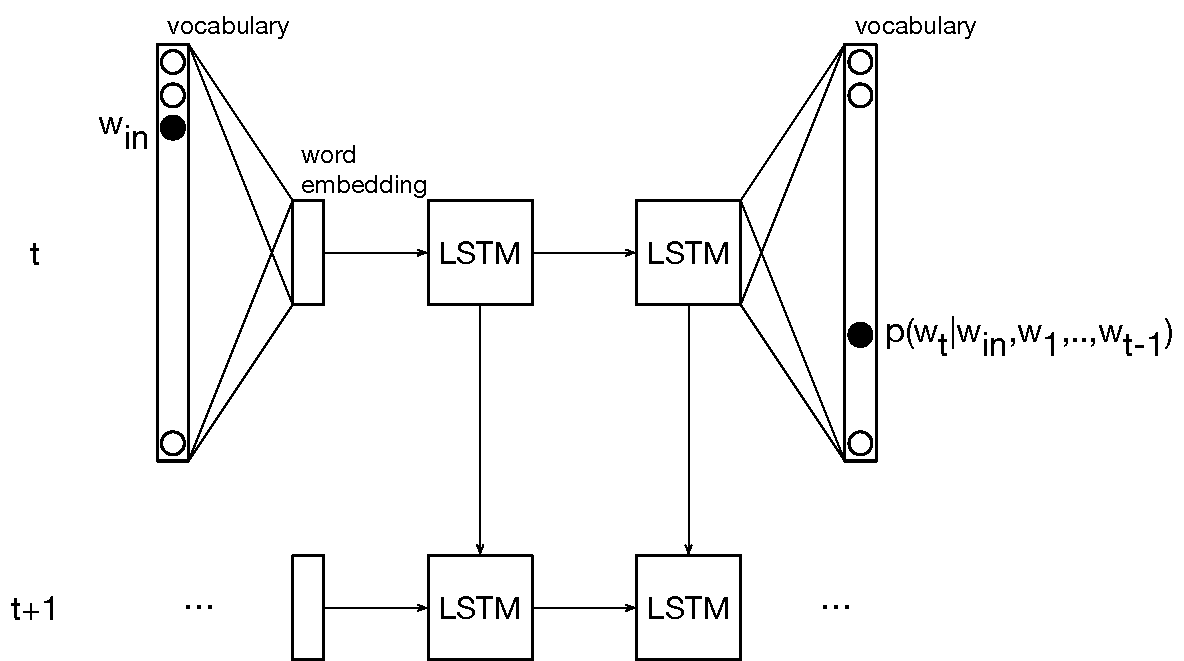
\includegraphics[width=\linewidth]{lstm-lm-small.pdf}
 \caption{Recurrent Neural Network language model architecture with LSTM units.}
 %\autoref{tab:vis_papers}. The image is from \cite{Isenberg:2017:VMC} and is in the public domain.}
 \label{fig:lstm_rnn}
\end{figure}

\begin{figure}[tb]
 \centering % avoid the use of \begin{center}...\end{center} and use \centering instead (more compact)
 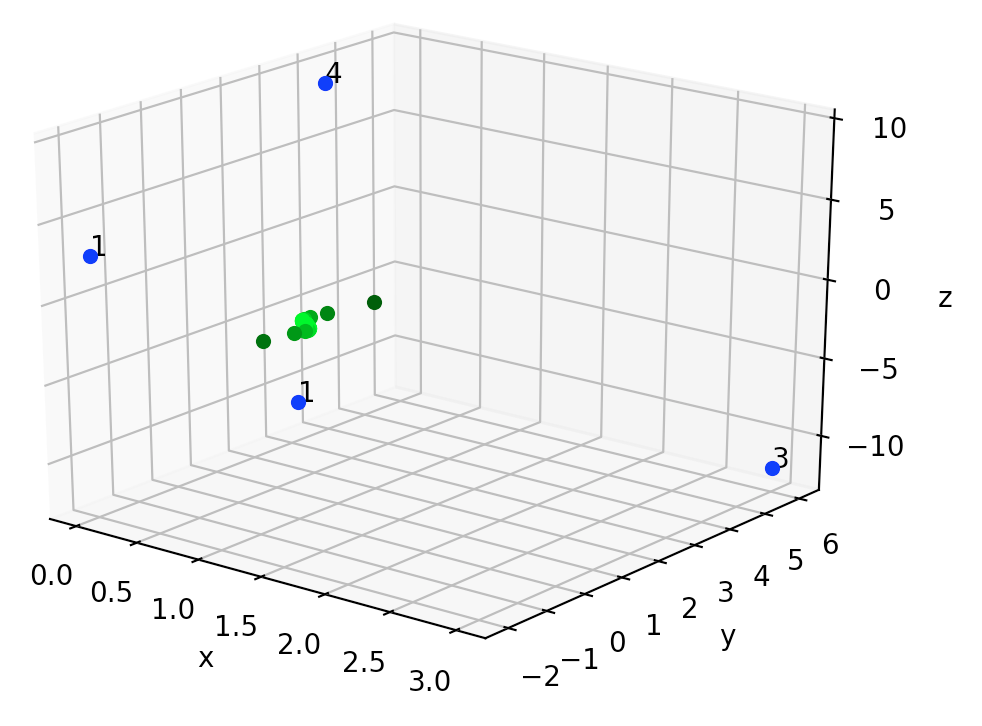
\includegraphics[width=\linewidth]{point_fitting.png}
 \caption{Fitting a point into 3D based off four reference points, with $d_{v_1}=1$, $d_{v_2}=1$, $d_{v_3}=3$, $d_{v_4}=4$.  As the iterations proceed, the point that starts out dark green becomes lighter and lighter green until convergence.}
 %\autoref{tab:vis_papers}. The image is from \cite{Isenberg:2017:VMC} and is in the public domain.}
 \label{fig:point_fitting}
\end{figure}

\end{document}


